%%%%%%%%%%%%%%%%%%%%%%%%%%%%%%%%%%%%%%%%%%%%%%%%%%%%%%%%%%%%%%%%%%%%
%% chapter5.tex
%% UNL thesis document file
%%
%% Chapter with lots of dummy text
%%%%%%%%%%%%%%%%%%%%%%%%%%%%%%%%%%%%%%%%%%%%%%%%%%%%%%%%%%%%%%%%%%%%
\chapter{Research Plan}
\label{cha:plan}
\acresetall

This final chapter aims in presenting the main tasks for this PhD based on the research questions from the introductory chapter:
\textit{\paragraph{Research question 1:} How can different modalities be represented mathematically in order to provide more insights of the relationship between speech disorders and expression of emotions then each modality by itself provides?}

\textit{\paragraph{Research question 2:} How can temporal progress of observed repeated experiments be evaluated in context of a multimodal framework?}
\\

In order to tackle \textbf{RQ 1}, first a multimodal framework is built based on available datasets (\textbf{Task I}). Then data is collected (\textbf{Task II}) and the created framework is applied on the data (\textbf{Task III}).

To answer \textbf{RQ 2} a second dataset needs to be collected over time (\textbf{Task IV}) and analyzed (\textbf{Task V}).

\paragraph{Task I - Create a baseline using existing datasets for multimodal analysis.}
By using existing datasets (See Table~\ref{tab:rgbDatasets}, \ref{tab:3DThermaldatasets} and chapter~\ref{subsec:multiDatasets}), a multimodal framework will be developed to relate data from different modalities. For that purpose different toolboxes (see chapter~\ref{sec:sensorsFeatures}) will be used to extract features from the different modalities and different data fusion methods will be explored. The different algorithms to extract features as well as to fuse the data will be integrated in one framework in order that it can be applied on various multimodal datasets to evaluate the performance of the system in different conditions.

\paragraph{Task II - Define a setup and experimental protocol and collect data from \gls{pws} or patients with \gls{pd} or \gls{ad} suffering \gls{dysarthria} or \gls{apraxia}, as well as from healthy adults as control group.}
Cooperation will be searched with experts mentioned in chapter~\ref{sec:experts} to define the experimental protocol and have access to patients. Voluntary subjects in the same age range will be recorded as control group.

\paragraph{Task III - Unimodal and multimodal analysis of the data collected} The framework developed in \textbf{Task I} will be used to analyze the collected data. Each modality will be analyzed separately as well as fused together (possible methods in chapter~\ref{sec:sensorsFeatures}). Obtained insights can be used to develop new algorithms in order to improve the mapping of visible facial muscle activity to correct/incorrect execution of speech exercises. The correlation of speech errors detected through video and audio analysis and the emotional inner state measured through \gls{eda} will be computed as well as correlation between the facial expressiveness and emotional inner state. 

\begin{comment}
\paragraph{Task IV - Analyze influence of emotional biofeedback in stutter therapy over time.} Existing therapy exercises will be combined with emotional biofeedback. Given the insights from \textbf{Task IIb}, the modalities which gather most information will be used to collect data during several therapy sessions. As the collected data will represent the progress over time, a mathematical framework will be developed to represent the evolution over time. This representation can be used to develop a measurement of the benefit the therapy provides.
\end{comment}

\paragraph{Task IV - Collect data during therapy sessions to analyze data over time.} Depending on the outcomes obtained in \textbf{Task III} patients can be accompanied during conventional therapy or a new therapy can be developed using emotional biofeedback, based on prior outcomes.

\paragraph{Task V - Analyze collected data over time.} Adapt multimodal framework to evaluate temporal progress of observed repeated experiments in context of a multimodal framework.


\begin{figure}
    \centering
    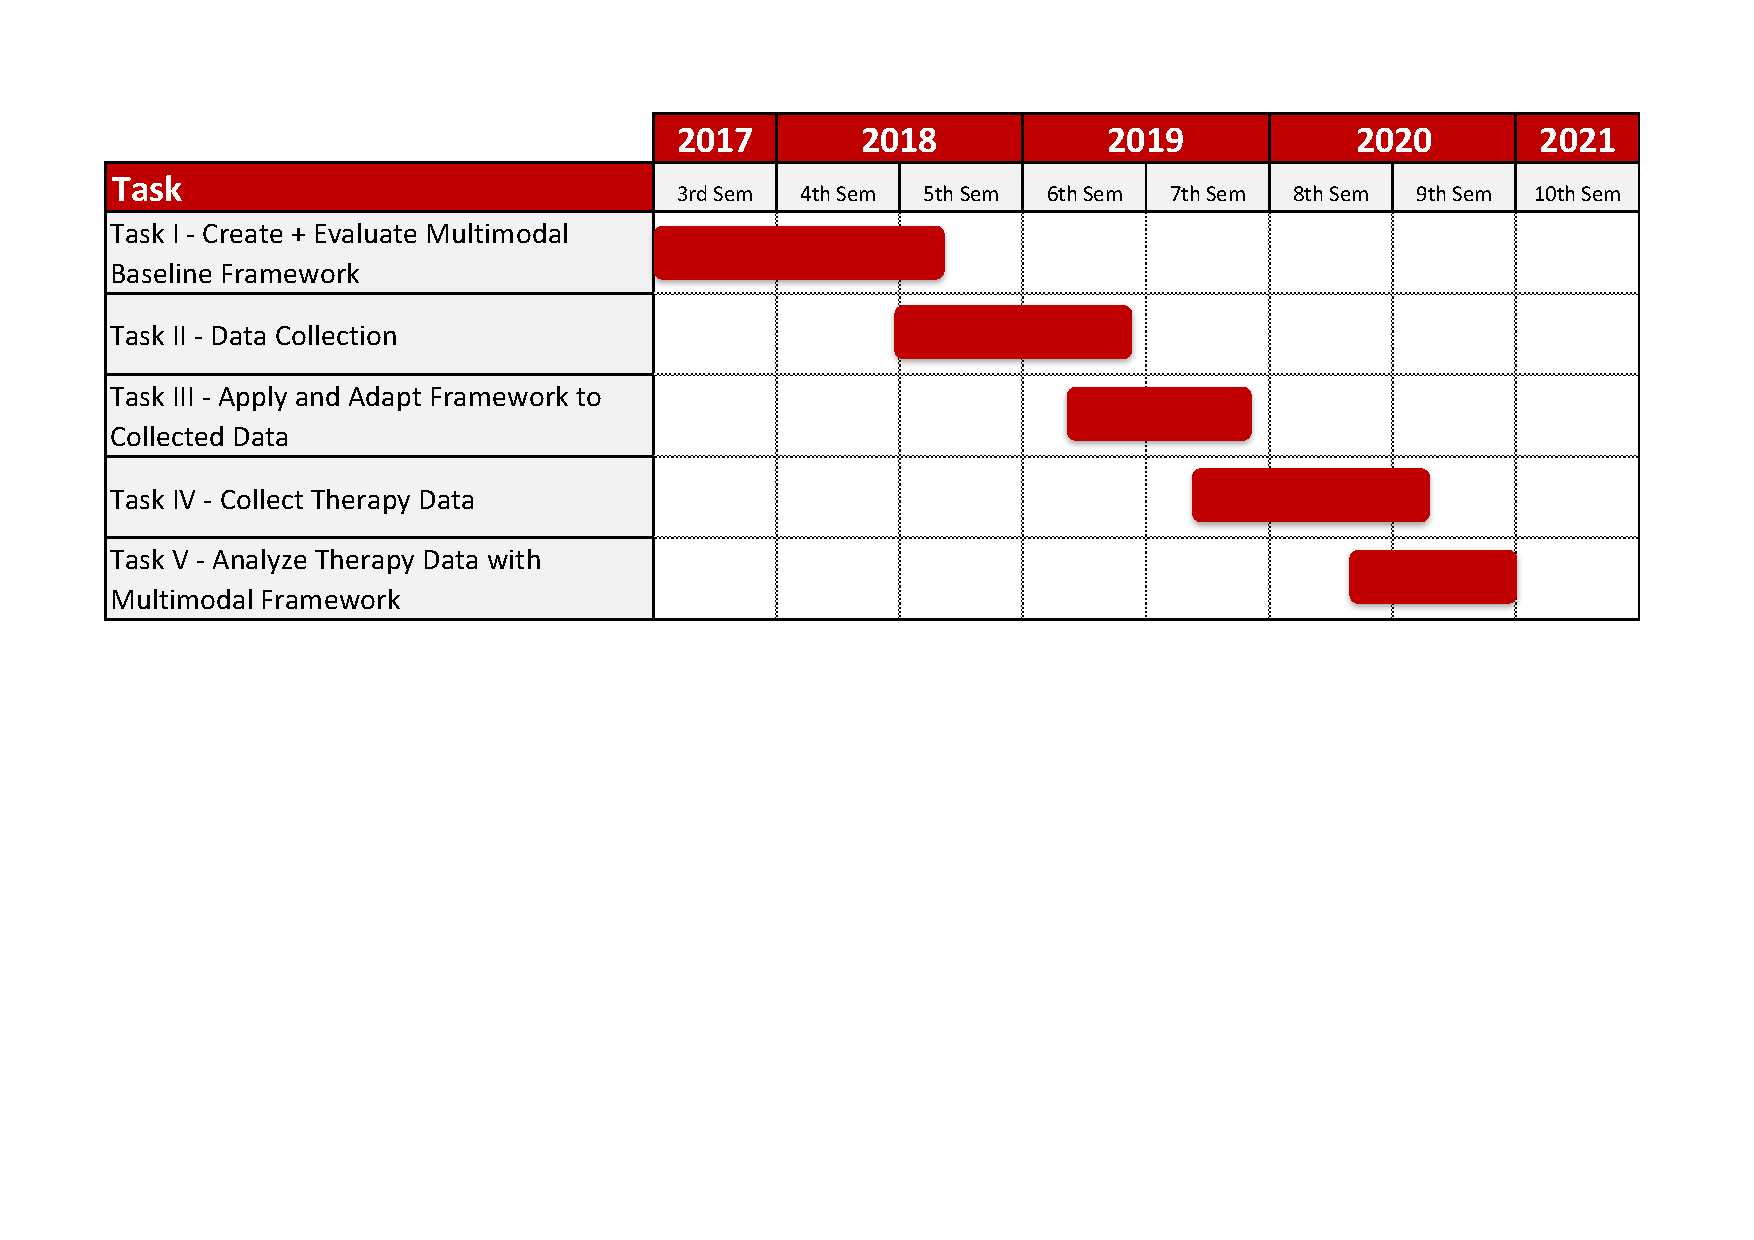
\includegraphics[width=14cm]{ganttChart}
    \caption{Time Plan for 2017-2021.}
    \label{fig:timePlan}
\end{figure}






\begin{comment}
\textbf{Task 1- Research image features for RGB, depth, and infrared data that permit the mapping of visible facial muscle activity to correct/incorrect execution of speech exercises OR paralysis severity.} It is expected that by combining different modalities (RGB, depth, infrared) the feature representation of facial activity is improved. The goal is that the feature representation permits the binary classification of correct/incorrect execution of speech exercises in the case of applying to speech therapy. In the case of facial paralysis the goal is to have a feature representation that permits a multiclass classification for the degree of severity of the paralysis.\\

\textbf{Task 2 - Understand the relation ... engagement during exercises through detecting relevant facial expressions.} Speech therapy requires monotonous repetition of exercises which can affect the engagement of the patient. By detecting in real-time the disengagement of the patient, different exercises can be suggested to maintain a positive learning curve. \\

\textbf{Task 3 - Research feature spaces that relates in meaningfully manner information from different modalities, therapist annotations and time.}
Suuport the SLTs reasoning and exploration of health data. 
Additionally to visual features, therapist annotations will be used to represent the progress of the therapy over time. As the therapy is performed through several sessions the time component is essential to measure the progress of a patient. 

\textbf{Task 4 - Develop statistical model that suggests future exercises by comparing one patient with similar ones in an existing database.} By being able to model the temporal progress of the therapy, the progress of one patient can be compared to the progress of others. Patients with similar starting point and positive conclusion of the therapy, can be taken as example and can provide insights of therapeutic actions that can help other similar patients to improve their progress. Thus, future actions to take can be suggested to the therapist. This model could also be used for other applications where temporal progression of a disease is observed through several therapy sessions. 


\end{comment}




